%==============================================================================%
%            PRØVE | FORKURS 1P-2P LÆRERUTDANNING | V2018 | UTSATT             %
%==============================================================================%
%
% __/\\\\\\\\\\\\____________________/\\\\\\___________________/\\\_
%  _\/\\\////////\\\_________________\////\\\_______________/\\\\\\\_
%   _\/\\\______\//\\\___________________\/\\\______________\/////\\\_
%    _\/\\\_______\/\\\_____/\\\\\\\\_____\/\\\__________________\/\\\_
%     _\/\\\_______\/\\\___/\\\/////\\\____\/\\\__________________\/\\\_
%      _\/\\\_______\/\\\__/\\\\\\\\\\\_____\/\\\__________________\/\\\_
%       _\/\\\_______/\\\__\//\\///////______\/\\\__________________\/\\\_
%        _\/\\\\\\\\\\\\/____\//\\\\\\\\\\__/\\\\\\\\\_______________\/\\\_
%         _\////////////_______\//////////__\/////////________________\///_
%
%==============================================================================%
%                              UTEN HJELPEMIDDEL                               %
%==============================================================================%
\Del{u}


%==============================================================================%
%                                 OPPGAVE 1.1                                  %
%==============================================================================%
\Oppgave[1] \points*{1}

\begin{figure}[H]
  \centering
  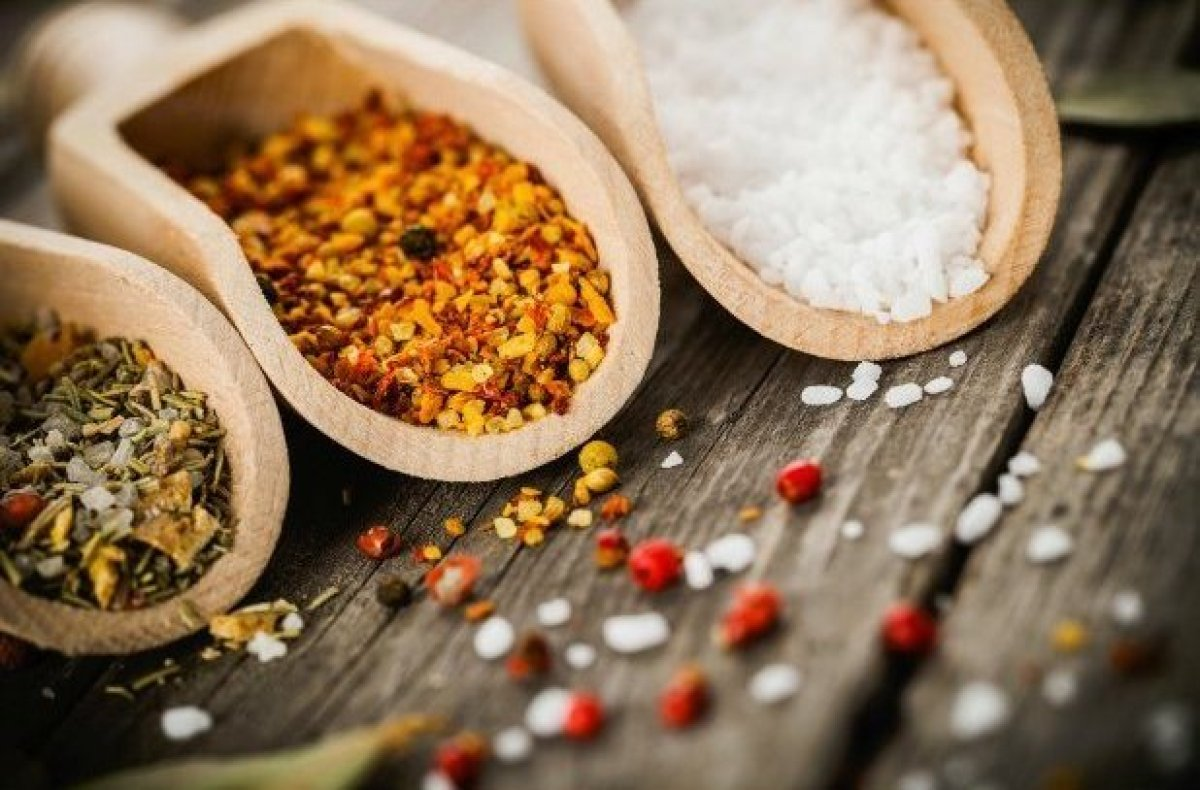
\includegraphics[width=0.7\linewidth]{Forkurs-1p-2p-laererutdanning-2018-V-U-oppgave-1-1-krydder.jpg}
\end{figure}

I $\SI{40}{\g}$ av en krydderblanding er det $\SI{16}{\g}$ salt. \medskip

Hvor mange prosent av krydderblandingen er salt?


%==============================================================================%
%                                 OPPGAVE 1.2                                  %
%==============================================================================%
\Oppgave[1] \points*{1}

I $1930$ var konsumprisindeksen 3, og i $1976$ var den $21$. \medskip

Hvor mange prosent økte prisene på varer og tjenester for en
gjennomsnittsfamilie i denne perioden?


%==============================================================================%
%                                 OPPGAVE 1.3                                  %
%==============================================================================%
\Oppgave[2] \points*{2}

Regn ut
%
\begin{equation*}
  \frac{\num{4.2e-4}+\num{6e-5}}{\num{200e-6}}
\end{equation*}


%==============================================================================%
%                                 OPPGAVE 1.4                                  %
%==============================================================================%
\Oppgave[2] \points*{2}

I $2010$ var indeksen for en vare $90$. Varen kostet da 540 kroner. I $2017$ var
indeksen for den samme varen $96$. \medskip

Hvor mye kostet varen i $2017$ dersom prisen har fulgt indeksen?


%==============================================================================%
%                                 OPPGAVE 1.5                                  %
%==============================================================================%
\Oppgave[3] \points*{3}

\begin{figure}[H]
  \centering
  \begin{subfigure}[b]{0.45\textwidth}
    \centering
    \tikzsetnextfilename{Forkurs-1p-2p-laererutdanning-2018-V-U-oppgave-1-5a}
    \begin{tikzpicture}[scale=0.5]
      \tkzInit[xmin=-5.1,xmax=0.1,ymin=-0.1,ymax=13.1]
      \tkzClip
      \edef\hypotenuse{13}
      \edef\longLeg{12}

      \tkzDefPoint(0,0){B}
      \tkzDefPoint(-1,0){b}
      \tkzDefPoint(0,\longLeg){C}

      \tkzInterLC[R](B,b)(C, \hypotenuse cm) \tkzGetPoints{a}{A}

      \tkzMarkRightAngle[thick, scale=4,color=maincolorMedium](A,B,C)
      \tkzDrawPolygon[thick,color=maincolorMedium](A,B,C)
    \end{tikzpicture}
    \caption{}
  \end{subfigure}%
  ~
  \begin{subfigure}[b]{0.45\textwidth}
    \centering
    % \tikzsetnextfilename{Forkurs-1p-2p-laererutdanning-2018-H-oppgave-1-5b}
    \begin{tikzpicture}[scale=0.5]
      % \tkzInit[xmin=-5.1,xmax=0.1,ymin=-0.1,ymax=13.1]
      % \tkzClip
      % \edef\hypotenuse{13}
      \edef\longLeg{12}
      \pgfmathsetmacro\radii{\longLeg*0.5}

      \tkzDefPoint(0,0){B}
      \tkzDefPoint(0,\longLeg){C}
      \tkzDefPoint(0,\longLeg/2){O}
      \tkzDrawArc[thick, color=maincolorMedium](O,B)(C)
      \tkzDrawSegment[thick, color=maincolorMedium](B,C)
    \end{tikzpicture}
    \caption{}
  \end{subfigure}%
  \caption{}
  \label{fig:Forkurs-1p-2p-laererutdanning-2018-V-U-oppgave-1-5}
\end{figure}

Gitt en rettvinklet trekant og en halvsirkel. Hypotenusen i trekanten er
$\SI{13}{\cm}$, og den lengste kateten er $\SI{12}{\cm}$. Radius i halvsirkelen
er $\SI{6}{\cm}$. Se
\cref{fig:Forkurs-1p-2p-laererutdanning-2018-V-U-oppgave-1-5}. \medskip

Gjør beregninger og avgjør hvilken av de to figurene som har størst omkrets.


%==============================================================================%
%                                 OPPGAVE 1.6                                  %
%==============================================================================%
\Oppgave[2] \points*{2}

\begin{minipage}{0.75\textwidth}
  Overflaten av en terning er $\SI{54}{\cm\squared}$. \medskip

  Hvor lange er sidekantene til terningen?
\end{minipage}
\begin{minipage}{0.25\textwidth}
  \begin{figure}[H]
    \includegraphics[width=0.75\linewidth,trim={12cm 0 0 0},clip]{%
      Forkurs-1p-2p-laererutdanning-2018-V-U-oppgave-1-6-dices.png%
    }
    \caption{}
    \label{fig:Forkurs-1p-2p-laererutdanning-2018-V-U-oppgave-1-6}
  \end{figure}
\end{minipage}


%==============================================================================%
%                                 OPPGAVE 1.7                                  %
%==============================================================================%
\Oppgave[4]

En butikk selger roser i vaser. Tabellen nedenfor viser sammenhengen mellom antall
roser i en vase, og samlet pris for vasen med rosene.

\begin{table}[H]
  \newcommand{\tbnum}[1]{\multirow{-2}{*}{#1}}
    \centering
    \caption{}
    \label{tab:Forkurs-1p-2p-laererutdanning-2018-V-U-oppgave-1-7}
    \begin{tabular}{| l | *{3}{r|} } \hline
      \Cellcolor{År}        &         15  &         21  &         35  \\ \hline
      \Cellcolor{Antall}    &             &             &             \\[-0.02cm]
      \Cellcolor{individer} & \tbnum{305} & \tbnum{377} & \tbnum{545} \\ \hline
    \end{tabular}
\end{table}

\begin{oppgaver}
  \Item{1} Hvor mye koster hver rose, og hvor mye koster selve vasen?
\end{oppgaver}

\begin{oppgaver}
  \Item{2} Bestem den lineære modellen som viser sammenhengen mellom antall
    roser i vasen og samlet pris for vasen med rosene.
\end{oppgaver}

Arne betaler $475$~kroner for en vase med roser.

\begin{oppgaver}
  \Item{1} Hvor mange roser har han i vasen?
\end{oppgaver}


%==============================================================================%
%                                 OPPGAVE 1.8                                  %
%==============================================================================%
\Oppgave[3] \points*{3}

I april i år målte Line temperaturen utenfor huset sitt hver morgen. Resultatene
ser du i tabellen nedenfor.

\begin{table}[H]
    \centering
    \caption{}
    \label{tab:Forkurs-1p-2p-laererutdanning-2018-V-U-oppgave-1-8}
    \begin{tabular}{|S[table-format=2.0] |S[table-format=1.0]|}
      \tableHeaders{Temperatur (\si{\celsius})}{Antall dager}
         -5 & 5 \\
         -3 & 4 \\
         -2 & 6 \\
          1 & 2 \\
          3 & 4 \\
          4 & 4 \\
          5 & 4 \\
          8 & 1 \\ \hline
    \end{tabular}
\end{table}

Bestem typetallet, medianen og gjennomsnittet for dette datamaterialet.


\newpage
%==============================================================================%
%                                 OPPGAVE 1.9                                  %
%==============================================================================%
\Oppgave[2]


\begin{figure}[H]
  \centering
  \tikzsetnextfilename{tab:Forkurs-1p-2p-laererutdanning-2018-V-U-oppgave-1-9}
  \begin{tikzpicture}
    \begin{axis}[
      Eksamen1,
      ytick={0,1,...,9},
      yticklabel = {\num{\fpeval{\tick*50}}},
      xtick={0,1,...,6},
      ymin=-.1,
      ymax=10,
      xmin=-.1,
      xmax=7,
      domain = 0:6,
      ]
      \addplot[color=maincolorMedium,thick,samples=250] {8*2^(-x)} node[right,pos=0.25] {$f$};
      \node[] at (axis cs: 3,9.5) {Pris per T-skjore (kroner)};
      \node[align=left] at (axis cs: 5.75,2.05) {Antall timer etter \\ klokka 20.00};

      \draw [maincolorMedium, fill] (axis cs: 0,8) circle (3pt) node [above
      right] {$(1, \num{400})$};
      \draw [maincolorMedium, fill] (axis cs: 1,4) circle (3pt) node [above right] {$(2, \num{200})$};
      \draw [maincolorMedium, fill] (axis cs: 2,2) circle (3pt) node [above
      right] {$(3, \num{100})$};
      \draw [maincolorMedium, fill] (axis cs: 3,1) circle (3pt) node [above
      right] {$(4, \num{50})$};
      \draw [maincolorMedium, fill] (axis cs: 4,0.5) circle (3pt) node [above
      right] {$(5, \num{25})$};
    \end{axis}
  \end{tikzpicture}
  \caption{}
  \label{fig:Forkurs-1p-2p-laererutdanning-2018-V-U-oppgave-1-9}
\end{figure}

Ovenfor i \cref{fig:Forkurs-1p-2p-laererutdanning-2018-V-U-oppgave-1-9} ser du
grafen til en eksponentialfunksjon $f$. Grafen viser prisen for
en T-skjorte $x$ timer etter klokka 20.00.

\begin{oppgaver}
  \Item{1} Hvor mye vil en T-skjorte koste når butikken stenger klokken $02:00$?
\end{oppgaver}

\begin{oppgaver}
  \Item{1} Bestem funksjonsuttrykket $f(x)$.
\end{oppgaver}


%==============================================================================%
%                                 OPPGAVE 1.10                                 %
%==============================================================================%
\Oppgave[4]

\begin{figure}[H]
  \centering
  \begin{subfigure}[b]{0.25\textwidth}
    \centering
    \tikzsetnextfilename{Forkurs-1p-2p-laererutdanning-2018-V-U-oppgave-1-10a}
    \drawCircles{1}
    \caption{}
    \label{subfig:Forkurs-1p-2p-laererutdanning-2018-V-U-oppgave-1-10a}
  \end{subfigure}\hfill%
  \begin{subfigure}[b]{0.32\textwidth}
    \centering
    \tikzsetnextfilename{Forkurs-1p-2p-laererutdanning-2018-V-U-oppgave-1-10b}
    \drawCircles{2}
    \caption{}
    \label{subfig:Forkurs-1p-2p-laererutdanning-2018-V-U-oppgave-1-10b}
  \end{subfigure}\hfill%
  \begin{subfigure}[b]{0.41\textwidth}
    \centering
    \tikzsetnextfilename{Forkurs-1p-2p-laererutdanning-2018-V-U-oppgave-1-10c}
    \drawCircles{3}
    \caption{}
    \label{subfig:Forkurs-1p-2p-laererutdanning-2018-V-U-oppgave-1-10c}
  \end{subfigure}
  \caption{}\label{fig:Forkurs-1p-2p-laererutdanning-2018-V-U-oppgave-1-10}
\end{figure}

Ovenfor ser du tre figurer. Figurene er satt sammen av små sirkler. Tenk deg at
du skal fortsette å lage figurer etter samme mønster.

\begin{oppgaver}
  \Item{3} Skriv av
  \cref{tab:Forkurs-1p-2p-laererutdanning-2018-V-U-oppgave-1-10}, og fyll ut det
  som mangler. Gjør beregninger, eller forklar hvordan du tenker.
\end{oppgaver}

\begin{table}[H]
  \centering
  \caption{}
  \label{tab:Forkurs-1p-2p-laererutdanning-2018-V-U-oppgave-1-10}
  \begin{tabular}{| S[table-format=1.0] | S[table-format=2.0] |}
    \tableHeaders{Figur}{Antall sirkler}
    1   &  9 \\
    2   & 12 \\
    3   & 16 \\
    4   &    \\
    5   &    \\
    {$n$} &    \\ \hline
  \end{tabular}
\end{table}

I en figur som er laget etter dette mønsteret er det $328$ lilla sirkler.

\begin{oppgaver}
  \Item{1} Hvor mange hvite sirkler er det i denne figuren?
\end{oppgaver}















